\chapter{Analysis}
\label{analysis}
This chapter discusses different approaches to fulfill the desired requirements. It also provides the arguments for the selection of some specific libraries later used in the Distrace tool. It starts with the section summarizing the limitations of the similar monitoring solutions and is followed by several sections where each of them is dedicated for a single requirement. There we discuss in more detail what solution is the best for meeting the desired requirement. This chapter ends with the summary of desired and unwanted features.

\section{Limitations of Similar Solutions}
In this thesis, we try to overcome some of the limitations of the relevant monitoring tools and give users the alternative solution. One goal of the Distrace tool is to be an open-source solution, which is in contrast to the proprietary Google Dapper described in Section \ref{dapper}. Google Dapper is also targeted to the only specific type of applications sharing the same code structure and libraries used at Google. Therefore, it can be said that there is a certain lack of the universality at Google Dapper. 

Zipkin, more described in Section \ref{zipkin}, is stable open-source tracing system. Zipkin creates several pre-instrumented libraries which may be used at the monitored application to communicate with the Zipkin backend. These libraries try to minimize a number of code changes in application sources, however, the user is still required to add custom annotations or change the default tracing mechanism. The similar holds for very similar HTrace tool which is described in more details in Section \ref{htrace}. HTrace also performs the instrumentation in the same JVM (Java Virtual Machine) where the application is running which can have a performance impact on the application itself.

The Distrace tool proposed by this thesis attempts to address these problems and find solutions how applications can be instrumented without the need of changing the source code and have the minimal performance impact on the running application. It, however, shares the same concepts as \textit{Span} and\textit{ Distributed traces} with the platforms already mentioned.
\section{Small Footprint and High Performance}
The mentioned cluster monitoring tools, such as Google Dapper and Zipkin, can affect the application performance and memory consumption since they perform instrumentation in the same virtual machine as the monitored application. One of the thesis requirements is to have minimal footprint on the monitored application.

Since the instrumentation is the core functionality of the system, it directly affects the performance of the application. Different instrumentation methods are discussed in the following few paragraphs to give the reader insights into how each method can affect the application's performance. Two standard ways of instrumentation exist - either using the native agent or Java agent. The advantages and disadvantages of these two approaches are discussed here together with the arguments for the final solution which is actually a compromise of both techniques.
\subsection{Java Agent}
\label{java_agent}
Java agents are used for instrumenting the applications on the Java language level, where the user does not need to worry about the JVM internals. For example, Byte Buddy, Javassist or CGLib may be used for this purpose. Usually, the programmer extends and creates custom class file transformers and the agent internals takes care of applying the code when required. 

The advantage of this approach is obvious - the ability to write the instrumentation in the high-level language without the knowledge of the underlying bytecode. The distributions of Java Agents is also platform independent since they are packaged inside JAR (Java ARchive) files as the rest of Java classes. 

The disadvantages of this approach are usually the performance and the flexibility of the agent. Objects created by Java agents are affected by garbage collection of the monitored application and thus can have a negative impact on the application itself. Also, the objects created from the agent are put on the application's heap and therefore consume the memory of the application. For the reasons above, it can happen that the observed information via Java Agent can be influenced by the monitoring process itself. Java agents also can not be used to respond to internal JVM events. It is important to note that Java system classes can not be instrumented when using this method.
\subsection{Native Agent}
Native agents are used for monitoring and instrumenting the applications in the low-level programming language (C, C++) using JVMTI and JNI. Native agents are written as native libraries for specific platforms and therefore the packaging is not platform independent. 

The disadvantage of this method can be that the agent has to be written in C or C++, but on the other hand, this approach gives the developer the full flexibility in the instrumentation and monitoring of the JVM state. For example, even the System classes can be instrumented using this approach and callbacks may be created to respond to several JVM internal events such as start or end of the garbage collection process, creation of a new instance of a specific class or thread switches. The native agent is running as part of the Java process and therefore any resource-demanding computation can have a negative performance impact on the application's performance as well as in the previous agent approach. However, objects created in the native agent are not subject to garbage collection and are not created on the heap, except when they are created using JNI in the target Java application.

The significant technical disadvantage of this approach is that it does not provide any helper methods to help with the code instrumentation and generally, there is a lack of stable instrumentation libraries written in C++ or C that could be used inside the agent. The developer of the native agent has to write all the required methods for extracting the relevant parts of the bytecode and the instrumentation itself.
\subsection{Chosen Method}
\label{subsec:inst_jvm}
The desired solution should be able to instrument the code without affecting the performance and memory of the monitored application whilst still having access to internal JVM state and allowing the developer to use a high-level programming language to write the instrumentation code. For these reasons, the compromise between the proposed approaches has been chosen, together with the introduction of the special Java process used specifically for the instrumentation. The solution can be seen in Figure \ref{fig:inst_server_basic}.
\begin{figure}
	\centering
	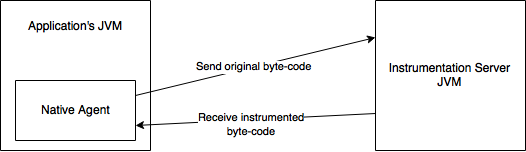
\includegraphics[scale=0.7]{inst_server.png}
	\caption{Sketch of the chosen approach.}
	\label{fig:inst_server_basic}
\end{figure}

In more detail, the native agent is used to communicate with the application being monitored. When a class needs to be instrumented, the native agent sends the class's bytecode to a special instrumentation server JVM. This machine handles the instrumentation and sends the instrumented bytecode back to the native agent. Therefore the native agent is only used for collecting important internal JVM information, sending classes for instrumentation and receiving the instrumented classes back. The instrumentation does not happen in the same JVM as the monitored application, which allows the tool to have a minimal performance impact on the application. Also, since the instrumentation is not done in the native agent, but in the instrumentation server based on Java, this machine can use any of the available bytecode manipulation tools which operate on Java language level and therefore, there is no need to implement the bytecode manipulation library completely from scratch in the native agent. Another advantage of this solution is that even the application's Java system classes may be instrumented in Java language on the instrumentation server.

Byte Buddy library was selected for the bytecode manipulation within the instrumentation server  as it allows to write the instrumentation in Java without the deep knowledge about the Java bytecode, which is necessary when using ASM library. Also, the library is supposed to have a really good performance results based on the benchmarks conducted by the author of the library \cite{ByteBuddy_Perf}. Compared to Javassist, the code is not written inside Java strings, which has the effect that the instrumentation code can be validated in today's IDE (Integrated Development Environment) during compilation time and bugs in the instrumentation code can be found easier. Compared to CGLib, the API of the library is well-documented and the library is under active development. Byte Buddy is also a highly configurable library, which was also the significant reason for choosing it as the tool for instrumenting classes inside different JVM than where they are actually used. Achieving the instrumentation in the secondary JVM  turned out to be challenging part of the thesis and the technical aspects of the solutions are described later in the thesis.

The disadvantage of the chosen approach is that the native agent has to send the bytecode to the instrumentation server and wait for the instrumented bytecode. However several optimizations have been implemented to minimize this delay as much as possible. More information about these optimizations can be found in Section \ref{sec:inst_server}
			
\subsection{Alternative solutions}
Two alternative instrumentation solutions were analyzed but rejected at the end. The first alternative solution was to perform the instrumentation right in the agent, even for the price of affecting the application's performance by instrumenting in the same JVM. However this solution required to write the instrumentation from scratch in C++ or C language, since there are no stable libraries for this purpose. Even though this would be possible, it would take a significant amount of time and also, it was not the goal of the thesis to create such a library. The performance impact on the application's was also the important reason for rejecting this method.

The other alternative solution was based on the idea of running multiple Java Virtual Machines inside one native process. In particular, that would mean running the application and the instrumentation server inside the same process. This would have the same  negative performance impacts as the solution above, however it would allow the developer to perform the instrumentation in Java programming language compared to C++ or C. Also all the communication between the machines would be only inside one single process compared to the chosen solution where the communication needs to be handled over the network or between different processes. However, as of JDK/JRE 1.2, creation of multiple virtual machines in a single process is not supported \cite{MoreJVMOnceProccess}.
							
\subsection{Chosen Communication Layer}
The selection of the tool used for the communication between the native agent and the instrumentation server was also important decision and we choose Nanomsg for the tool purposes. Comparing to raw sockets approach, Nanomsg hides the platform specific aspects of the socket communication. It has also several performance benefits and general improvements over the well-known ZeroMQ library, such as better threading and more sophisticated implementation of the zero-copy technique. The mappings of this library into Java and C++ languages mentioned in Section \ref{nanomsg} were also perfect fit into the tool.
		

\section{Transparency and Universality}
One of the most important goals of the thesis is to achieve high level of application transparency while ensuring the tool universality. Each of these two requirements directly affects the second one and therefore we needed to find compromise between these two.


The rejected approach was to create an universal monitoring tool similar to Google Dapper, but allow to monitor mostly shared aspects of distributed applications. This solution would give the user great flexibility, universality and would also ensure that users don't need to extend the library. However, implementing such a solution was decided as not a feasible task. Every platform or application is different in its architecture or in the way how it communicates and therefore identifying the shared parts between all distributed applications is an extremely challenging task. Also, such instrumentation tool could only instrument very basic information about Java-based programs.

The architecture of the chosen approach can be seen in Figure \ref{fig:extending_core}. The chosen approach for the monitoring tool was to design it as an general extendable instrumentation library with two kinds of users - developer and end user. The tool should be available as a library with well-defined methods for defining the instrumentation points and specifying the custom annotations. The developer of the application is responsible for extending this library and based on it, create application-specific monitoring tool. Therefore, the developer has to have understanding of the monitored application and has to know the type of information, which are to be collected. The developer also takes care of defining where a new span starts and when existing span ends. The end-user of this final library is just responsible for starting the application with the monitoring tool attached and does not need to understand the application internals.

The advantage of this approach is that only core instrumentation library needs to be created that is universal and generic to all Java-based applications. On the other hand, the application's developer is required to extend the library in order to provide the desired monitoring functionality. However, for this price, the original application can remain unchanged and from the end-user point of view, the monitoring tool is completely transparent to the monitored application.

In more detail, the core monitoring library acts as the instrumentation server mentioned in the previous section. It can be seen in Figure \ref{fig:extending_core} that by extending the core library, the developer creates an application-specific instrumentation server, which specifies the parts of the original application to be instrumented. The application-specific instrumentation server then communicates with the native agent, which is universal to all Java applications. It is important to mention that the instrumentation server is used only for instrumentation. The instrumented code is responsible for storing data to the user interface.
\begin{figure}
	\centering
	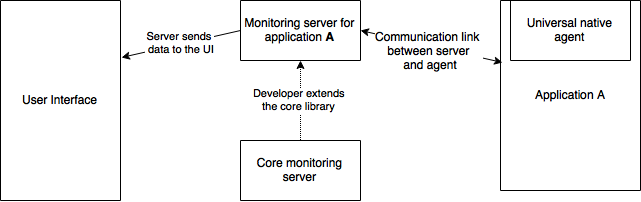
\includegraphics[scale=0.5]{extending_core.png}
	\caption{.}
	\label{fig:extending_core}
\end{figure}


\section{Easiness of Use}
This requirement is highly connected to the previous one. The easiness of use is also important goal of the application. The usage of the core monitoring system is separated into two user groups, developers and end users. The goal is to not require from the end user to know the internal structure of the application and the monitoring platform. This is achieved by assuming that the developer, who is responsible for extending the library, can handle this technicalities. The user is supposed to work with the user interface and to read the results of the monitoring run. 

However, it is also our goal to ensure that the developer responsible for extending the core monitoring tool needs to write a few lines of code as possible and does not need to have a deep knowledge about the JVM internals or application bytecode. This is also the reason why Java language and Byte Buddy library are used for the instrumentation on the server. The Byte Buddy library provides several very concise ways how to define the application-specific instrumentation. To shield the developer from the internals, all low-level core code is hidden from the developer in the native agent, which is universal to all Java applications and the developer is not supposed to change its implementation.

\section{Easiness of Deployment}
In order to ensure the easiness of deployment, the number of artifacts used by the tool should be as low as possible. Also the application should have understandable and relatively small configuration so the users can effectively set up the application for their desired needs. 

Based on the discussion in the previous sections, the tool should have only two final artifacts - the universal native agent and the core monitoring server, which is supposed to be extended by the application developer for specific application needs.

The deployment of this tool should be also simplified at certain use-cases by starting the application-specific instrumentation server automatically from the native agent. In most cases, the user should only specify path to the instrumentation library and attach the native agent to the application. Several deployment strategies exist and are discussed later in the thesis.

\section{Modularity}
It is the also goal of the tool to allow the user to replace some of the default application modules of the whole platform by specific custom modules without the need of rewriting the complete application.

The extendable modules should be the interface presenting the observed data and the collectors bringing the data from the application nodes to the user interface. Whilst default implementation are available in the tool, the users have the possibility to plug-in custom user interface or more advanced data collectors. The modules have to meet some specific criteria in order to replace the default implementations, however the core implementation is left up to the user. 

The main reason for this solution is that a lot of monitoring frameworks already exist. For example, an user interface provided by some different tool may be already deployed or some platform with already defined data collection may be used. The thesis tries to support these use-cases and tries to minimize the changes of the environment where this monitoring tool runs. This also leads to easier deployment of the platform. 

\subsection{Selection of the User Interface}
Zipkin user interface was selected as the default user interface for the Distrace tool. The main reasons for its selection were the simplicity of the interface and ease of use. It also fulfills our visualization requirements as it allows the user to see dependencies between spans and also whole trace tree as well. However, as mentioned above, the monitoring platform is not tightly-coupled to this user interface. It is described later in the thesis how the user can create a plug-in allowing to use custom user interface.

\section{Summary of Features}
This section just summarize the list of desired and not-desired features based on the previous background and analysis.

Desired features and properties of the thesis based on the analysis are:
\begin{itemize}
	\item Ability to collect distributed traces and spans via the instrumentation.
	\item Native agent implemented in C++ to be attached to a Java application. The native agent is universal to all Java applications and is not supposed to be changed.
	\item Instrumentation server implemented in Java used for the instrumentation. The instrumentation server acts as the core library, which can be extended by the application's developer for the specific application. Byte Buddy library is to be used within the server for the code transformations and definitions of the instrumentation points.
	\item Nanomsg library is to be used as the communication layer between the native agent and the instrumentation server.
	\item Support for the Zipkin user interface. The user interface is used to visualize the collected spans.
	\item Ability to replace the default user interface with the custom user interface.
\end{itemize}

Selected features and properties which are not desired by this thesis:
\begin{itemize}
	\item Support for creating a custom user interface. 
	\item Support for creating an universal instrumentation tool, which would not require the developer to specify the instrumentation points and specify start and end of spans.
	\item Implementing bytecode instrumentation in C++.
	\item Instrumenting the Java bytecode in the same machine as the running application.
\end{itemize}

